\chapter{Evaluation}
\label{chap:evaluation}

\glsreset{mae}
\glsreset{mse}
\glsreset{rmse}
\glsreset{r2}
% \glsresetall

This chapter thoroughly illustrates the evaluation of our generalization strategy by comparing the three model variants proposed in section \ref{sec:model-variants}. The measurement includes both quantitative and qualitative evaluations. On one side, a quantitative valuation provides numerical results, which are crucial for scientifically assessing the network's capabilities through a set of chosen metrics. On the other side, qualitative observations rely on human interpretation to evaluate models' possible behaviors in some real contexts.

The first part of this chapter focuses on the application of statistical metrics for quantitatively examine the three models both on the training (section \ref{sec:evaluation-training}) and the test set (section \ref{sec:evaluation-quantitative}). The former is used to briefly understand overall models' learning, while the latter aims to present unseen examples to the network to estimate its generalization capabilities.

An official test set is made available by Mantegazza et al. \cite{mantegazza2019visionbased}. For enhancing testing capabilities, we take advantage of background replacement to generate artificial datasets from the test set. Notice that image manipulation can cause unrealistic patterns in the data, leading to potential biases during the evaluation. Nonetheless, the background replacement technique allows us to perform quantitative evaluations without the need of recording new data in different environments. 


\subsection{Metrics}
\label{subsec:metrics}

The following list presents an overview of all the principal metrics adopted for our evaluation and used in the next sections.

\begin{itemize}
	\item \gls{mae} measures the average residuals in the dataset, which means the absolute difference between the actual and predicted values. The lower the \gls{mae}, the better the model. Assuming $y_i$ as the predicted value and $\hat{y_i}$ as the ground truth, the \gls{mae} is defined as follows:
	$$ MAE = \frac{1}{N} \sum_{i=1}^N |y_i - \hat{y_i}| $$
	
	\item \gls{rmse} measures the standard deviation of residuals. As for \gls{mae}, \gls{rmse} should be as lower as possible. It penalizes large prediction errors, thus is not particularly suited to be used on a dataset with many outliers. The main advantage and reason for its usage in evaluating regression models is because \gls{rmse} has the same unit as the dependent variable, so it is easy to interpret.
	$$ RMSE = \sqrt{\frac{1}{N} \sum_{i=1}^N (y_i - \hat{y_i})^2} $$
	
	\item \gls{r2} (or coefficient of determination) measures the robustness of the regression. It represents the proportion of the variance in the dependent variable which is explained by the independent variable. \gls{r2} is often the best choice for evaluating regression performance because it provides a measure of fitness for the model to predict unseen data correctly. Also, its domain is easily understandable since it goes from $-\infty$ to 1: an optimal model (with no prediction errors) will have an \gls{r2} of 1; a model that always predicts the average value will have an \gls{r2} of 0; a model worse than the average predictor will have a negative \gls{r2}. Considering $\overline{y}$ the mean value:
	$$ R^2 = 1 - \frac{\sum_{i=1}^N (y_i - \hat{y_i})^2}{\sum_{i=1}^N (y_i - \overline{y})^2} $$
\end{itemize}




\section{Training Results}
\label{sec:evaluation-training}

As for the entire chapter, this section considers the \texttt{Arena}, \texttt{CVPR} and \texttt{CVPR Aug} models defined in section \ref{sec:model-variants}. Here, we introduce their performance during the training procedure presented in section \ref{sec:implementation-training}.

In this phase, the loss function (\gls{mae}) and the \gls{r2} score are take into consideration, both for the train and the validation set. Figures \ref{fig:training-metrics-arena}, \ref{fig:training-metrics-cvpr} and \ref{fig:training-metrics-cvpraug} show metrics evolution over the 60 training epochs. Overall, it can be said that at least 30 epochs are needed to reach convergence, after which the performance stabilizes.

\texttt{Arena}, \texttt{CVPR}, and \texttt{CVPR Aug} achieve a validation loss of 0.07, 0.13 and 0.20, respectively. As the model complexity increases, the loss does. However, with data augmentation, the gap between training and validation loss significantly decreases, as shown in figure \ref{fig:training-metrics-cvpraug}. This may be a symptom of better generalization capabilities, although we do not yet have enough information to draw a conclusion on the subject. Even though the \texttt{CVPR Aug} model appears to improve by further increasing the number of epochs, experiments with 200 epochs have substantially the same results as 60.

The \texttt{Arena} model registers an \gls{r2} of 0.99, which can be attributable to overfitting. In fact, such a score would be obtained by an optimal model, but we already know that the original FrontalNet by \cite{mantegazza2019visionbased} could not properly operate outside of the drone arena. In the next sections, we will examine models \texttt{CVPR} and \texttt{CVPR Aug} on various test sets to certify their robustness against the \texttt{Arena} one.

\begin{figure}[H]
	\centering
	\includegraphics[width=1 \textwidth]{"contents/images/06-training-arena"}
	\caption[\texttt{Arena} model's performance during training. Loss and \gls{r2} on training and validation sets]{\texttt{Arena} model's performance during training. Loss and \gls{r2} on training and validation sets}
	\label{fig:training-metrics-arena}
\end{figure}

\begin{figure}[H]
	\centering
	\includegraphics[width=1 \textwidth]{"contents/images/06-training-CVPR"}
	\caption[\texttt{CVPR} model's performance during training. Loss and \gls{r2} on training and validation sets]{\texttt{CVPR} model's performance during training. Loss and \gls{r2} on training and validation sets}
	\label{fig:training-metrics-cvpr}
\end{figure}

\begin{figure}[H]
	\centering
	\includegraphics[width=1 \textwidth]{"contents/images/06-training-CVPRaug"}
	\caption[\texttt{CVPR Aug} model's performance during training. Loss and \gls{r2} on training and validation sets]{\texttt{CVPR Aug} model's performance during training. Loss and \gls{r2} on training and validation sets}
	\label{fig:training-metrics-cvpraug}
\end{figure}




\section{Quantitative Evaluation}
\label{sec:evaluation-quantitative}

Performance reported during training is not sufficient to evaluate the model. Its strengths must be measured on previously unseen data, but the validation set is very similar to the training one.

For testing, we first rely on the official test set \cite{mantegazza2019visionbased}. Then, we expand it through background replacement, choosing the two indoor scenarios shown in figure \ref{fig:test-indoor}. They do not belong to the CVPR dataset and have been accurately selected to be challenging enough for the model while somehow allowing a person in them to be easily recognized. The respective datasets, created by replacing all the test images backgrounds, are called \texttt{indoor1} and \texttt{indoor2}. Instead, we call \texttt{arena} the original test set.

\begin{figure}[!h]
	\begin{center}
		\begin{subfigure}[h]{0.49\textwidth}
			\centering
			\includegraphics[width=1\textwidth]{"contents/images/06-indoor1"}
		\end{subfigure}
		\hfill
		\begin{subfigure}[h]{0.49\textwidth}
			\centering
			\includegraphics[width=1\textwidth]{"contents/images/06-indoor2"}
		\end{subfigure}
	\end{center}
	\vspace{-0.5cm}
	\caption[Indoor backgrounds for quantitative evaluation]{Indoor backgrounds for quantitative evaluation}
	\label{fig:test-indoor}
\end{figure}

For a complete analysis, we test our three model variants (section \ref{sec:model-variants}) on the three test sets defined above. Again, we choose to compare the loss (\gls{mae}) and the \gls{r2} score. As previously explained in section \ref{subsec:metrics}, \gls{r2} represents the proportion of variance in the target (i.e., the user's pose) that is explained by the model features (i.e., the input image). As such variance is dataset dependent, \gls{r2} may not be meaningfully comparable across different datasets. Thus, the metric can only be compared among different models for the same dataset, but not on different data for the same model.

Unlike for training, during testing, we evaluate the \gls{r2} score separately on each variable, allowing us to inspect models' behavior further. Besides, we compute \gls{rmse}, particularly useful for understanding the errors' magnitude.

Results are shown in table \ref{tab:qt-summary} and summarized below. 

\paragraph*{Arena model evaluation}

This represents the baseline performance on the test set. On its native dataset (i.e., the \texttt{arena} test set) the loss is 0.41 and \gls{r2} lies between 0.74 and 0.86. As expected according to our previous knowledge on model performance out of the drone arena, also on background-replaced test sets the model behavior is very poor. On the \texttt{indoor1} dataset, the loss is 0.86 and the \gls{r2} scores ranges between 0.08 and 0.30. Even worse, on \texttt{indoor2} the loss is 1 and \gls{r2} registers negative values for variables \texttt{X} and \texttt{Z}.

\paragraph*{CVPR model evaluation}

The model trained on the background-replaced dataset is much better than the first when predicting the user's pose with unknown backgrounds. \texttt{CVPR} performance on \texttt{arena} test set are very similar to the one obtained on it by the \texttt{Arena} model. The loss is just 0.01 higher and the only big difference is found for the \texttt{X} \gls{r2}, which decreases from 0.81 to 0.69. Howbeit, the \texttt{indoor1} and \texttt{indoor2} test sets both registers similar performance for this model, with a loss of 0.44 and 0.45, respectively.

\paragraph*{CVPR Aug model evaluation}

Image augmentation seems to provide not only general improvements but also leverages the outcome for all variables. The \texttt{CVPR Aug} model achieves an \gls{r2} score greater of 0.80 for each variable on every test set. Moreover, its performance on the \texttt{arena} test set is the best so far, with a loss of 0.36. Relative \gls{r2} scores go from 0.75 to 0.87, encountering no particular differences among different test sets.

\paragraph*{Notes on variables}

Overall, all the models have consistent trends \gls{wrt} their variables. In all cases, the \texttt{W} \gls{rmse} is considerably higher than the others, and accordingly lower is its \gls{r2}. Also, \texttt{Z} \gls{rmse} is particularly low because of its distribution rather than actual good predictions. In fact, its \gls{r2} is lower than \texttt{Y} \gls{r2} even if the apparent squared error is better.

According to the coefficient of determination, \texttt{Y} and \texttt{Z} are the best predicted variables, followed by \texttt{X}. On the latter, image augmentation gives a huge advantage to the \texttt{CVPR Aug} model. 


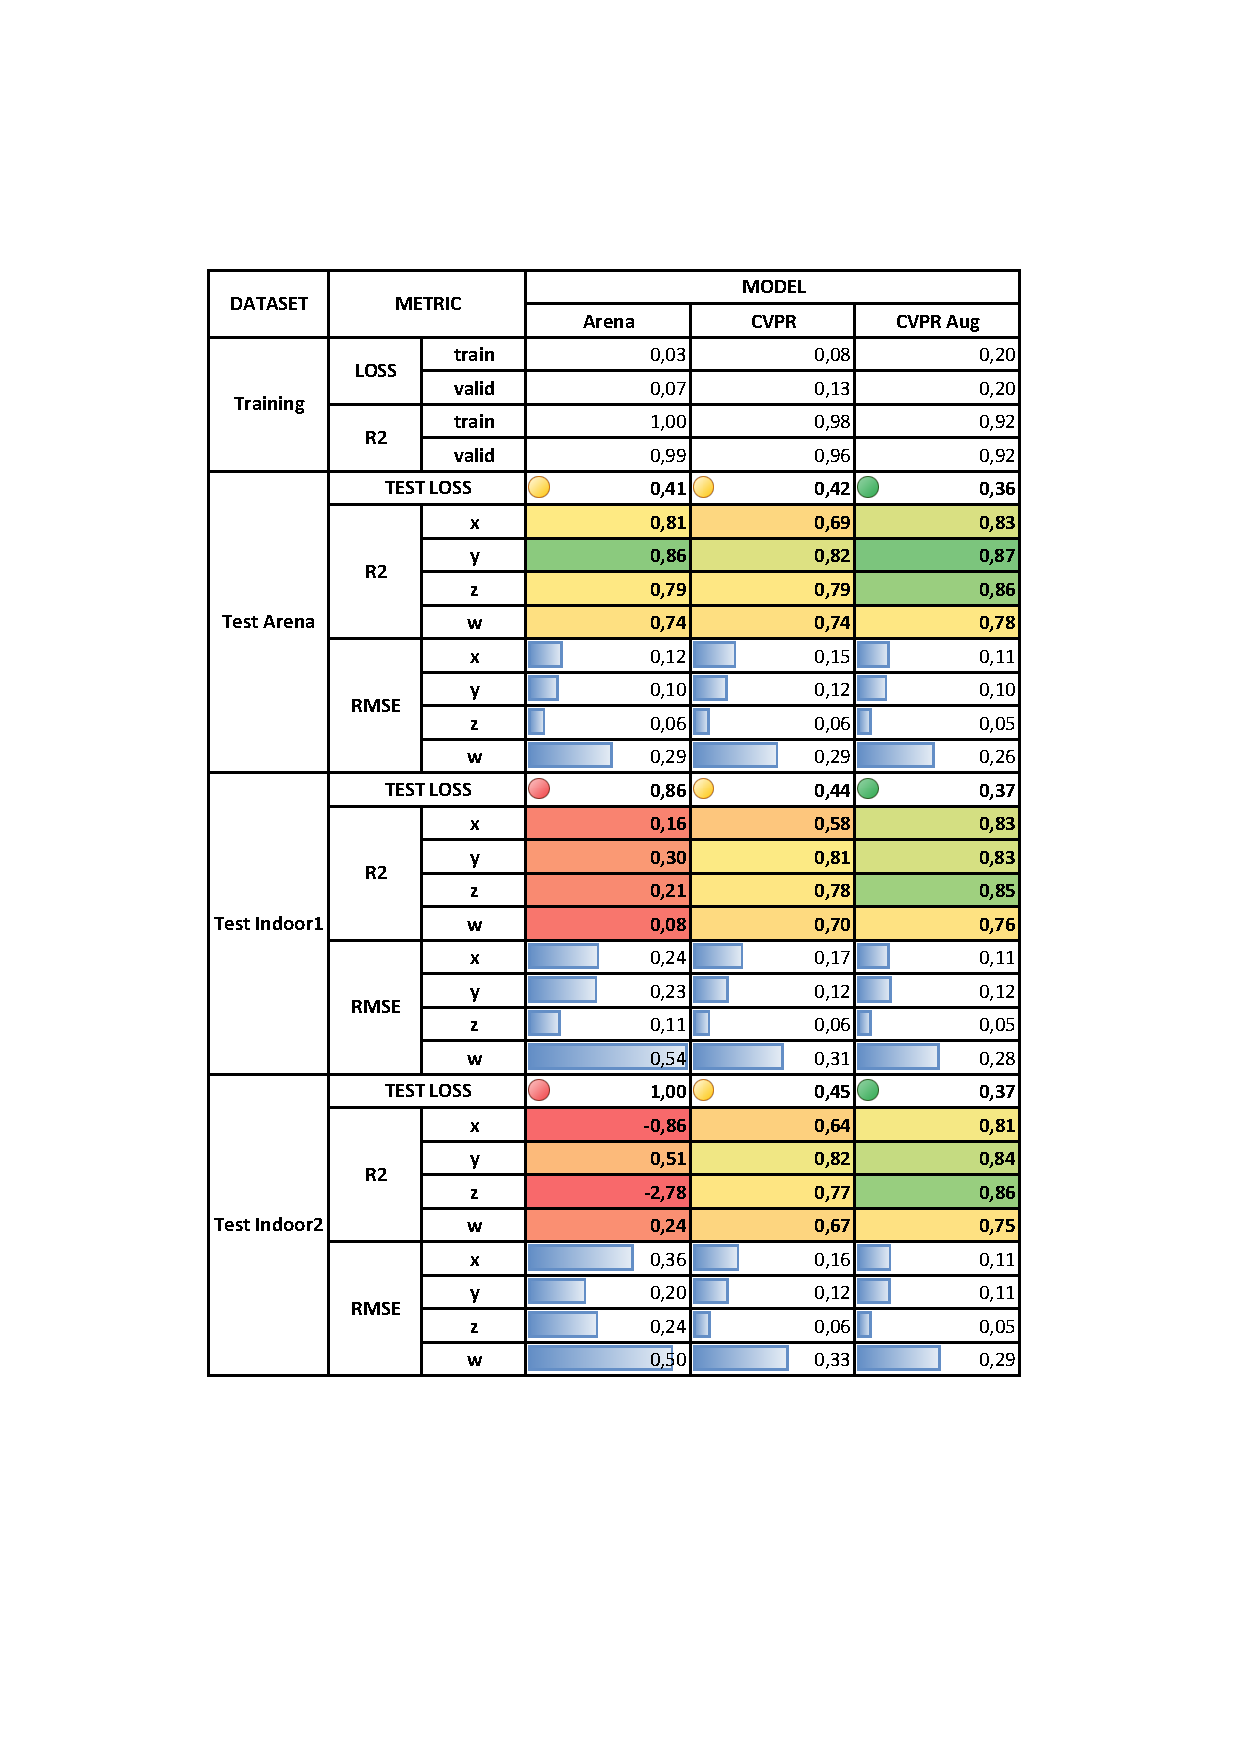
\includepdf[pages={1}, pagecommand={\null\vfill\captionof{table}{Quantitative evaluation: \texttt{Arena}, \texttt{CVPR}, \texttt{CVPR Aug} models on \texttt{arena}, \texttt{indoor1}, \texttt{indoor2} test sets.}\label{tab:qt-summary}}]{contents/images/06-qt-summary}


\subsubsection*{Final considerations on quantitative evaluation}

Considering the resulting metrics, it appears that our strategy undoubtedly improves the original model from a numerical perspective. The approach seems able to uncouple the training images from the generalized task of recognizing the user's position. Data augmentation plays a fundamental role in enhancing the robustness of the model. The \texttt{CVPR Aug} model, tested inside the drone arena, even produces better theoretical results than the original model. The reason is probably that such an environment is fairly easy to handle compared to the CVPR backgrounds, used during training, which are usually complex and sometimes tough to interpret even by humans.

To validate the results and extend the reasoning over numbers, a qualitative evaluation must be performed.



\section{Qualitative Evaluation}
\label{sec:evaluation-qualitative}

In this section, we do not consider precise metrics for assessing the model's fitness. Instead, we rely on simulation to create various visualizations and produce a behavioral evaluation of the results. In practice, we confront the models' predictions with the ground truth from a qualitative viewpoint.

A first evaluation, detailed in \ref{subsec:ql-timeline}, presents the comparison with timeline charts to investigate the general trend of each model on different test sets.

Next, in \ref{subsec:ql-interactive}, we make use of interactive visualizations that display the current frame, the predictions, and the ground truth altogether. These are used to interpret, from a human perspective, the models' results on specific images.



\subsection{Timeline comparison}
\label{subsec:ql-timeline}

\begin{figure}[H]
	\centering
	\includegraphics[width=1 \textwidth]{"contents/images/06-gtpred-arena"}
	\caption[Qualitative evaluation: \gls{gt} vs. predictions results on the \texttt{arena} test set]{Qualitative evaluation: \gls{gt} vs. predictions results on the \texttt{arena} test set}
	\label{fig:ql-gtpred-arena}
\end{figure}

\begin{figure}[H]
	\centering
	\includegraphics[width=1 \textwidth]{"contents/images/06-gtpred-indoor1"}
	\caption[Qualitative evaluation: \gls{gt} vs. predictions results on the \texttt{indoor1} test set]{Qualitative evaluation: \gls{gt} vs. predictions results on the \texttt{indoor1} test set}
	\label{fig:ql-gtpred-indoor1}
\end{figure}

\begin{figure}[H]
	\centering
	\includegraphics[width=1 \textwidth]{"contents/images/06-gtpred-indoor2"}
	\caption[Qualitative evaluation: \gls{gt} vs. predictions results on the \texttt{indoor2} test set]{Qualitative evaluation: \gls{gt} vs. predictions results on the \texttt{indoor2} test set}
	\label{fig:ql-gtpred-indoor2}
\end{figure}

\begin{figure}[H]
	\centering
	\includegraphics[width=1 \textwidth]{"contents/images/06-gtpred-mixed"}
	\caption[Qualitative evaluation: \gls{gt} vs. predictions results on the \texttt{mixed} test set]{Qualitative evaluation: \gls{gt} vs. predictions results on the \texttt{mixed} test set}
	\label{fig:ql-gtpred-mixed}
\end{figure}




\subsection{Per-frame comparison}
\label{subsec:ql-interactive}


